% Template for ICASSP-2016 paper; to be used with:
%          spconf.sty  - ICASSP/ICIP LaTeX style file, and
%          IEEEbib.bst - IEEE bibliography style file.
% --------------------------------------------------------------------------
\documentclass[12pt]{article}
\usepackage{spconf, amsmath, graphicx, float}
\usepackage{scrlayer-scrpage}
\clearpairofpagestyles
\cfoot*{\pagemark}
% Example definitions.
% --------------------
\def\x{{\mathbf x}}
\def\L{{\cal L}}

% Title.
% ------
\title{Moive Recommender System}
%
% Single address.
% ---------------
\name{Atom Group: Jifu Zhao (jzhao59), Jinsheng Wang (jwang278)}
\address{Nuclear, Plasma, and Radiological Engineering \\
              University of Illinois at Urbana-Champaign\\
		       Urbana, Illinois 61801, USA}

\begin{document}
%\ninept
%
\maketitle

\section{Introduction}
\quad\ In this project, our goal is to build a recommender system based on the MovieLens 1M Dataset. MovieLens 1M dataset contains 1,000,209 anonymous rating of approximately 3,900 movies made by 6,040 MovieLens users who joined MovieLens in 2000. These movies can be categorized into 18 different categories. In this project, based on some well developed Python package, we compared the performance of different algorithms and finally chose 2 models as our final models. More details will be described in the following sections.

\section{Pre-processing}
\quad\ The dataset has three files: movies.dat, ratings.dat and users.dat. Among these three files, the most useful one is the ratings.dat. Since the algorithm is pretty straightforward, there is little pre-processing steps. In this project, we compared the implementation and performance of Python and R, but finally we decided to use Python. The main package we used is called $ \textbf{surprise} $, a widely used Python package for building and analyzing recommender systems.

\section{Methods}

\quad\ $ \textbf{Surprise} $ has many algorithms, such as baseline algorithms, neighbourhood methods, matrix factorization-based (SVD, PMF, SVD++, NMF) and so on. In this project we first studied the performance of 10 different algorithms (NormalPredictor, BaselineOnly, KNNBasic, KNNWithMeans, KNNBaseline, SVD, SVDpp, NMF, SlopeOne, CoClustering). Through 5 folder cross validation, we finally chose two best performed algorithm: KNN with Means and naive SVD algorithms.

\subsection{KNN with Means Algorithm}
\quad\ KNN with Means algorithm basically is a collaborative filtering algorithm. It takes into account the mean ratings of each user. Two important factors for this algorithm are whether or not it is user-based and how to measure the similarity. With cross validation, we chose the mean squared difference (MSD) similarity and used item-based mode.

\subsection{SVD Algorithm}
\quad\ The SVD algorithm is popularized by Simon Funk during the Netflix Prize. In $ \textbf{Surprise} $, there are in fact two algorithms based on SVD: SVD and SVD++. Although SVD++ performs a little bit better than naive SVD algorithm, it takes too much longer time to run. So, in this project, we only implemented the naive SVD algorithm.

\section{Code Description}
\quad\ All of our code is contained in the file named \textit{mymain.py}. Firstly, It will read in the training and testing data. After building the KNN and SVD models, it will make predictions on the testing data set and save the prediction result into local csv files.

The code runs very fast. As tested, the total running time is around 3 minutes.

\section{Results}
\quad\ In this project, we use the Root-Mean-Square-Error (RMSE) as the metric to measure the performance of different algorithms. A summary of the result of 5 folder cross validation is shown in Table~\ref{result}.


\begin{table}[htb]
 \caption{Summary of Cross Validation} \label{result}
 \vspace{0.1in}
\begin{center}
  \begin{tabular}{  c  c  c}
    \hline
    RMSE/Model            & KNNWithMeans        & SVD     \\ \hline
    Fold 1                    & 0.8852                    & 0.8617 \\ \hline
    Fold 2                    & 0.8862                    & 0.8627 \\ \hline
    Fold 3                    & 0.8873                    &0.8627 \\ \hline
    Fold 4                    & 0.8866                    & 0.8625 \\ \hline
    Fold 5                    & 0.8830                    & 0.8603 \\ \hline
    Average                 & 0.8857                    &  0.8620 \\ \hline      
  \end{tabular}
\end{center}
\end{table}

Note: in our cross validation, the data was randomly splitted into 5 folders. But for actual testing, there will be some users or movies never shown up in training data set. In that case, the performance is expected to be a little bit worse.

The code descripted above was tested on our laptop, the average running time was about 3 minutes. The corresponding computer system is:
MacBook Pro, 2.6GHz Intel Core i7, 16 GB memory.  

\subsection*{Acknowledgement}

%\begin{figure}[htb]
%\centering
%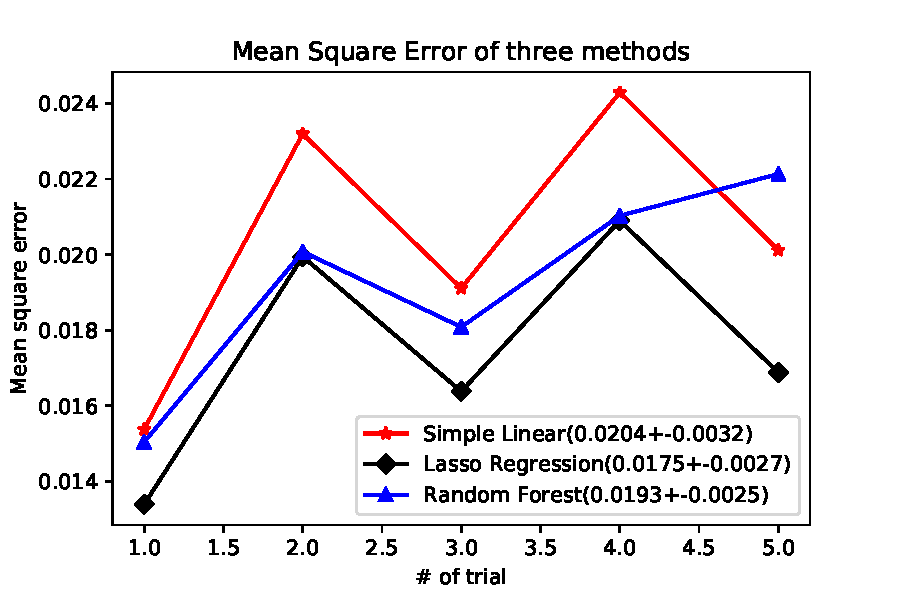
\includegraphics[width=0.45\textwidth]{./figures/MSE_3_methods.pdf}
%\caption{Results of different models}
%\label{fig:autoencoder}
%\end{figure}

\quad\ The authors would like to thank Xichen Huang for his tutorial notebook on Piazza.

\vfill\pagebreak

% References should be produced using the bibtex program from suitable
% BiBTeX files (here: strings, refs, manuals). The IEEEbib.bst bibliography
% style file from IEEE produces unsorted bibliography list.
% -------------------------------------------------------------------------
%\bibliographystyle{IEEEbib}%\bibliography{strings,refs}
%\bibliography{strings}

\end{document}